\subsection{Unified Table}

With the information we have found above, we must build a unified table
so we can plot the function accurately and conveniently.

\begin{center}
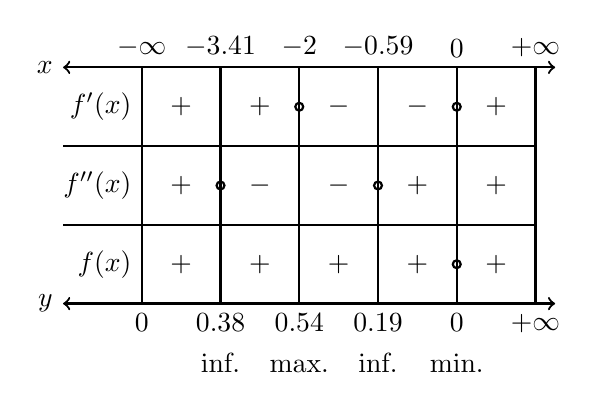
\begin{tikzpicture}
    \draw[thick, <->] 
        (0,0) -- (6.25,0)
        node [left] at (0,0) {$x$}
        node [above] at (1,0) {$-\infty$}
        node [above] at (2,0) {$-3.41$}
        node [above] at (3,0) {$-2$}
        node [above] at (4,0) {$-0.59$}
        node [above] at (5,0) {$0$}
        node [above] at (6,0) {$+\infty$};
    
    \draw[thick, <->]
        (0,-3) -- (6.25, -3)
        node [left] at (0,-3) {$y$}
        node [below] at (1,-3) {$0$}
        node [below] at (2,-3) {$0.38$}
        node [below] at (3,-3) {$0.54$}
        node [below] at (4,-3) {$0.19$}
        node [below] at (5,-3) {$0$}
        node [below] at (6,-3) {$+\infty$}
        ;
    \draw[thick]
        (1,0) -- (1,-3)
        (2,0) -- (2,-3)
        (3,0) -- (3,-3)
        (4,0) -- (4,-3)
        (5,0) -- (5,-3)
        (6,0) -- (6,-3)

        (0,-1) -- (6, -1)
        (0,-2) -- (6, -2)

        node [left] at (1, -0.5) {$f'(x)$}
        node [left] at (1, -1.5) {$f''(x)$}
        node [left] at (1, -2.5) {$f(x)$}
        ;
    
    \draw [thick]
        (3, -0.5) circle [radius=0.5mm]
        (5, -0.5) circle [radius=0.5mm]
        
        node at (1.5, -0.5) {$+$}
        node at (2.5, -0.5) {$+$}
        node at (3.5, -0.5) {$-$}
        node at (4.5, -0.5) {$-$}
        node at (5.5, -0.5) {$+$};
    
    \draw [thick]
        (2, -1.5) circle [radius=0.5mm]
        (4, -1.5) circle [radius=0.5mm]
        
        node at (1.5, -1.5) {$+$}
        node at (2.5, -1.5) {$-$}
        node at (3.5, -1.5) {$-$}
        node at (4.5, -1.5) {$+$}
        node at (5.5, -1.5) {$+$};
    
    \draw [thick]
        (5, -2.5) circle [radius=0.5mm]
        
        node at (1.5, -2.5) {$+$}
        node at (2.5, -2.5) {$+$}
        node at (3.5, -2.5) {$+$}
        node at (4.5, -2.5) {$+$}
        node at (5.5, -2.5) {$+$};
    
    \draw
        node [above] at (2,-4) {inf.}
        node [above] at (3,-4) {max.}
        node [above] at (4,-4) {inf.}
        node [above] at (5,-4) {min.};
    
\end{tikzpicture}
\end{center}

Now we have all the information we need for a plot of the graph.